\documentclass[12pt]{article}
\usepackage[a4paper]{geometry}
\usepackage[utf8]{inputenc}
\usepackage[myheadings]{fullpage}
\usepackage{fancyhdr}
\usepackage{lastpage}
\usepackage{float}
\usepackage{graphicx, wrapfig, subcaption, setspace, booktabs}
\usepackage{graphicx}
\usepackage[T1]{fontenc}
\usepackage[font=small, labelfont=bf]{caption}
\usepackage{fourier}
\usepackage[protrusion=true, expansion=true]{microtype}
\usepackage[english]{babel}
\usepackage{sectsty}
\usepackage{url, lipsum}
\usepackage[T1]{fontenc}
\usepackage{icomma}
\usepackage{ragged2e}
\usepackage{amsmath}
\usepackage{comment}
\usepackage{color}
\usepackage{xcolor}
\usepackage{listings}


\lstdefinelanguage{Golang}%
{morekeywords=[1]{package,import,func,type,struct,return,defer,panic,%
 recover,select,var,const,iota,},%
morekeywords=[2]{string,uint,uint8,uint16,uint32,uint64,int,int8,int16,%
 int32,int64,bool,float32,float64,complex64,complex128,byte,rune,uintptr,%
 error,interface},%
morekeywords=[3]{map,slice,make,new,nil,len,cap,copy,close,true,false,%
 delete,append,real,imag,complex,chan,},%
morekeywords=[4]{for,break,continue,range,go,goto,switch,case,fallthrough,if,%
 else,default,},%
morekeywords=[5]{Println,Printf,Error,Print,},%
sensitive=true,%
morecomment=[l]{//},%
morecomment=[s]{/*}{*/},%
morestring=[b]',%
morestring=[b]",%
morestring=[s]{`}{`},%
}

%New colors defined below
\definecolor{codegreen}{rgb}{0,0.6,0}
\definecolor{codegray}{rgb}{0.5,0.5,0.5}
\definecolor{codepurple}{rgb}{0.58,0,0.82}
\definecolor{backcolour}{rgb}{0.95,0.95,0.95}
%Code listing style named "mystyle"
\lstdefinestyle{mystyle}{% define my own style. Lots of options to choose from.
  backgroundcolor=\color{backcolour},   commentstyle=\color{codegreen},
  keywordstyle=\color{magenta},
  numberstyle=\tiny\color{codegray},
  stringstyle=\color{codepurple},
  basicstyle=\footnotesize,
  breakatwhitespace=false,
  breaklines=true,
  captionpos=t, %caption position t or b
  keepspaces=true,
  numbers=left,
  numbersep=5pt,
  showspaces=false,
  showstringspaces=false,
  showtabs=false,
  tabsize=2
}
\lstset{style=mystyle} %set the new style
\lstset{%aboveskip=\baselineskip, %don't want this aboveskip because it would put a
% space between our custom caption and the code.
belowskip=\baselineskip}

\newcommand{\HRule}[1]{\rule{\linewidth}{#1}}
\onehalfspacing
\setcounter{tocdepth}{5}
\setcounter{secnumdepth}{5}

%-------------------------------------------------------------------------------
% HEADER & FOOTER
%-------------------------------------------------------------------------------
\pagestyle{fancy}
\fancyhf{}
\setlength\headheight{15pt}

\begin{document}

\begin{titlepage}
  \title{ \normalsize \textsc{BlockChain and Cryptocurrencies}
      \\ [2.0cm]
      \HRule{0.5pt} \\
      \LARGE \textbf{\uppercase{HyperLedger POC}}
      \HRule{2pt} \\ [0.5cm]
      \normalsize \today \vspace*{5\baselineskip}}

  \date{}

  \author{
      Josef Dvořák \\
      Jiří Kalas \\
      Tomáš Přikryl }

  \thispagestyle{empty}
  \maketitle
  \thispagestyle{fancy}
\end{titlepage}
\newpage

\tableofcontents
\newpage

\section{Blockchain and network configuration}

Our implementation is available here: \url{https://github.com/imposis/fabric-samples/tree/test/project-network}.

In this POC we set up a blockchain network with two organizations.
Before a chaincode is deployed, it is first in the proposal phase.
We use a majority endorsement policy, which means that the chaincode is only committed and deployed if it is approved by the majority of peers.
After it is approved, the chaincode it then committed and deployed to the network.

In the implementation we had to store private data of the certificate holders securely. For this purpose we used the Hyperledger Fabric's private data collections.
\begin{figure}[H]
    \centering
    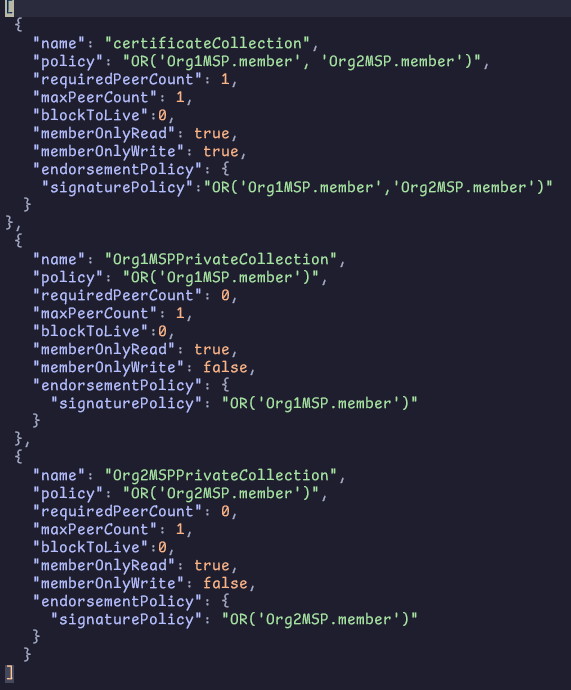
\includegraphics[width=0.6\textwidth]{imgs/collection_json.PNG}
    \caption{Collection definitions}
    \label{fig:collection}
\end{figure}

Here we defined a public collection shared between both organizations. Where members have both read and write permissions.
Then we defined a private collection for each organization. Which only members of that organization can access, which is used for storing private data of the certificate holder.

\newpage

\section{Chaincode implementation}
The chaincode definition is available here: \url{https://github.com/imposis/fabric-samples/blob/test/project-network/chaincode-go/certificate_operations.go}.

\subsection{Certificate structure}

\begin{lstlisting}[language=Golang]
type Certificate struct {
	Type            string `json:"objectType"`
	CertificateId   string `json:"certificateId"`
	NameSurname     string `json:"nameSurname"`
	CertType        string `json:"certType"`
	CertDescription string `json:"certDescription"`
	ValidFrom       string `json:"validFrom"`
	ValidUntil      string `json:"validUntil"`
	Owner           string `json:"owner"`
}

type CertificatePrivateDetails struct {
	CertificateId string `json:"certificateId"`
	UID           string `json:"UID"`
}
\end{lstlisting}

These 2 go structs describe the fields that are stored in the public and private data collections respectively. All fields are read as strings.
ValidFrom and ValidUntil are then converted to dates using the format yyyy-mm-dd.
When creating the certificates it is checked that validFrom is before validUntil.
The certificateId field is not generated by the network, but it should be generated by the client.
This is done to avoid race conditions that could occur when there is heavy traffic and the network could generate the same id twice.
When it is passed from client application we can check if the block containing the id exists in the ledger.

\subsection{SmartContract interface}

\begin{lstlisting}[language=Golang]
func (s *SmartContract) CreateCertificate(ctx contractapi.TransactionContextInterface) error
func (s *SmartContract) ChangeCertificateValidUntil(ctx contractapi.TransactionContextInterface, certificateId string, validUntil string) error
func (s *SmartContract) ReadCertificate(ctx contractapi.TransactionContextInterface, certificateId string) (*Certificate, error)
func (s *SmartContract) ReadCertificatePrivateDetails(ctx contractapi.TransactionContextInterface, collection string, certificateId string) (*CertificatePrivateDetails, error)
func (s *SmartContract) RemoveCertificate(ctx contractapi.TransactionContextInterface, certificateId string) error
\end{lstlisting}

These methods, defined for the SmartContract interface are available for use for operations on the blockchain.

\begin{itemize}
    \item \texttt{CreateCertificate} - method is used to create a new certificate. Based on the user stores private data to the collection of the organization of the user.
    \item \texttt{ChangeCertificateValidUntil} - method is used to change the validUntil field of the certificate. This is used to extend or reduce the validity of the certificate.
    \item \texttt{ReadCertificate} - method is used to read the public data of the certificate. Reads from the public collection.
    \item \texttt{ReadCertificatePrivateDetails} - method is used to read the private data of the certificate. Data stored only in the private collection of the organization of the user. Returns empty response when called by another organization
    \item \texttt{RemoveCertificate} - method is used to remove the certificate from the blockchain.
\end{itemize}

\subsection{Helper functions}

\begin{lstlisting}[language=Golang]
func getCollectionName(ctx contractapi.TransactionContextInterface) (string, error)
func verifyClientOrgMatchesPeerOrg(ctx contractapi.TransactionContextInterface) error
func submittingClientIdentity(ctx contractapi.TransactionContextInterface) (string, error)
\end{lstlisting}

\begin{itemize}
    \item \texttt{getCollectionName} - returns the private collection name of the organization of the user.
    \item \texttt{verifyClientOrgMatchesPeerOrg} - verifies that the organization of the user matches the organization of the peer.
    \item \texttt{submittingClientIdentity} - returns the id of the used who invoked the transation.
\end{itemize}

These functions are used in the SmartContract interface methods. Providing a functionality that can is used in multiple methods.

\newpage

\section{Example use}

Here we show an example use of the chaincode. The commands used are available here: \url{https://github.com/imposis/fabric-samples/blob/test/project-network/run.sh}

\subsection{Starting network and deploying chaincode}

First we need to start the network.

\begin{lstlisting}[language=bash]
./network.sh up createChannel -ca mychannel -s couchdb
\end{lstlisting}

Then we can deploy the chaincode.

\begin{lstlisting}[language=bash]
./network.sh deployCC -ccn private -ccp ../project-network/chaincode-go/ -ccl go -ccep "OR('Org2MSP.peer','Org2MSP.peer')" -cccg ../project-network/chaincode-go/collections_config.json
\end{lstlisting}

This does many steps that are needed to be split up later for production use, but in this POC it shows all the necessary steps that lead to the successful deployment of the chaincode.

First it publishes the chaincode in the proposal phase.
Then it needs to be approved by both organizations. In this example it needs to be approved by both organizations, because of the majority endorsement policy.
When there is more than 2 organizations, the chaincode needs to be approved by more than 50\% of the organizations.

\begin{figure}[H]
    \centering
    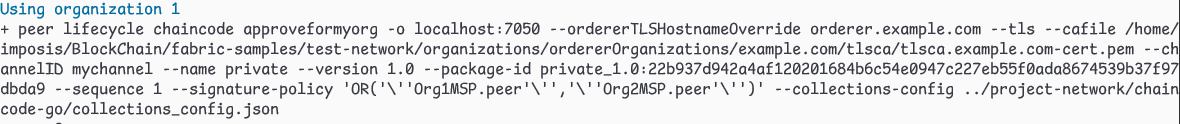
\includegraphics[width=\textwidth]{imgs/org1_approval.PNG}
    \caption{Org1 approval}
    \label{fig:org1approval}
\end{figure}

\begin{figure}[H]
    \centering
    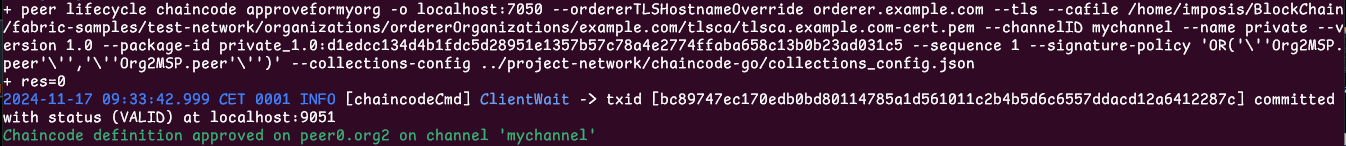
\includegraphics[width=\textwidth]{imgs/org2_approval.PNG}
    \caption{Org2 approval}
    \label{fig:org1approval}
\end{figure}

\begin{figure}[H]
    \centering
    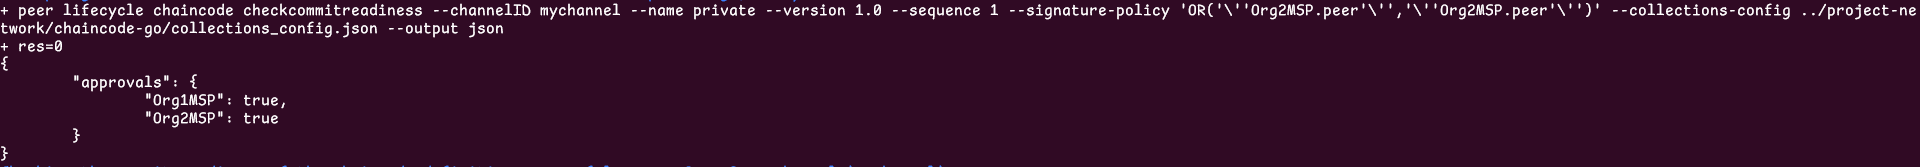
\includegraphics[width=\textwidth]{imgs/checking_approval.PNG}
    \caption{Checking approval}
    \label{fig:checkingapproval}
\end{figure}

After it is approved, the chaincode is then committed to the peers.

\begin{figure}[H]
    \centering
    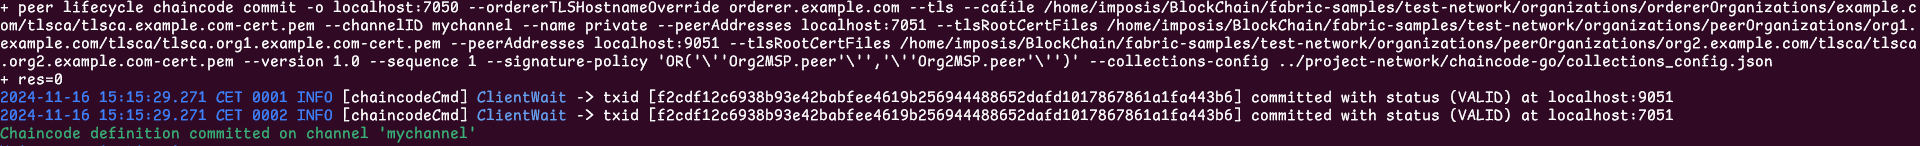
\includegraphics[width=\textwidth]{imgs/commiting_chaincode.PNG}
    \caption{Committing chaincode}
    \label{fig:commitingchaincode}
\end{figure}

After the chaincode is committed, it is available for use.

We also create certificates for both organizations, which are used for validation of the certificate ownership. This is done as described in the Hyperledger documentation.

\subsection{Certificate creation}

First we create a certificate.

\begin{lstlisting}[language=bash]
export CERT_PROPERTIES=$(echo -n "{ \"objectType\": \"certificate\", \"certificateId\": \"certificate1\", \"nameSurname\": \"John Doe\", \"certType\": \"IT\", \"certDescription\": \"IT certificate very nice\", \"validFrom\": \"2024-01-01\", \"validUntil\": \"2025-01-01\", \"UID\": \"990101/1234\" }" | base64 | tr -d \\n)
peer chaincode invoke -o localhost:7050 --ordererTLSHostnameOverride orderer.example.com --tls --cafile "${PWD}/organizations/ordererOrganizations/example.com/orderers/orderer.example.com/msp/tlscacerts/tlsca.example.com-cert.pem" -C mychannel -n private -c '{"function":"CreateCertificate","Args":[]}' --transient "{\"certificate_properties\":\"$CERT_PROPERTIES\"}"
\end{lstlisting}

Here we defined a certificate as a base64 encoded JSON object which is then passed to the CreateCertificate method.

\begin{figure}[H]
    \centering
    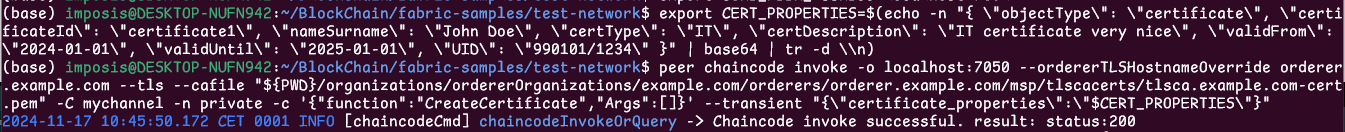
\includegraphics[width=\textwidth]{imgs/creating_certificate.PNG}
    \caption{Creating certificate}
    \label{fig:creatingcertificate}
\end{figure}

\subsection{Certificate reading as member of Org1}

Then we can read the certificate. Here is the result as member of Org1.

\begin{lstlisting}[language=bash]
peer chaincode query -C mychannel -n private -c '{"function":"ReadCertificate","Args":["certificate1"]}'
peer chaincode query -C mychannel -n private -c '{"function":"ReadCertificatePrivateDetails","Args":["Org1MSPPrivateCollection","certificate1"]}'
\end{lstlisting}

\begin{figure}[H]
    \centering
    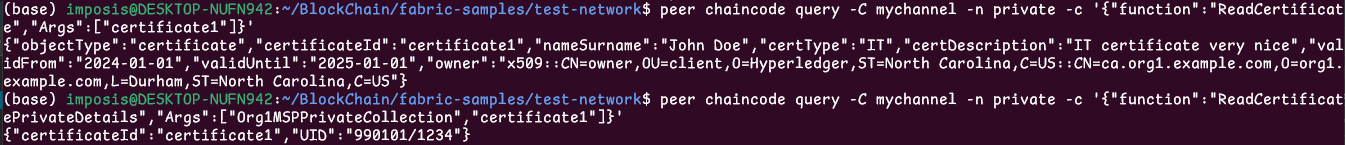
\includegraphics[width=\textwidth]{imgs/reading_certificate_org1.PNG}
    \caption{Reading certificate Org1}
    \label{fig:readingcertificate}
\end{figure}

As we can see the certificate is stored in the public collection, which doesn't include the private UID of the certificate holder.
When \texttt{ReadCertificatePrivateDetails} is called, the private data is returned.

\subsection{Certificate reading as member of Org2}

Here is the result as member of Org2.

\begin{lstlisting}[language=bash]
peer chaincode query -C mychannel -n private -c '{"function":"ReadCertificate","Args":["certificate1"]}'
peer chaincode query -C mychannel -n private -c '{"function":"ReadCertificatePrivateDetails","Args":["Org2MSPPrivateCollection","certificate1"]}'
peer chaincode query -C mychannel -n private -c '{"function":"ReadCertificatePrivateDetails","Args":["Org1MSPPrivateCollection","certificate1"]}'
\end{lstlisting}

\begin{figure}[H]
    \centering
    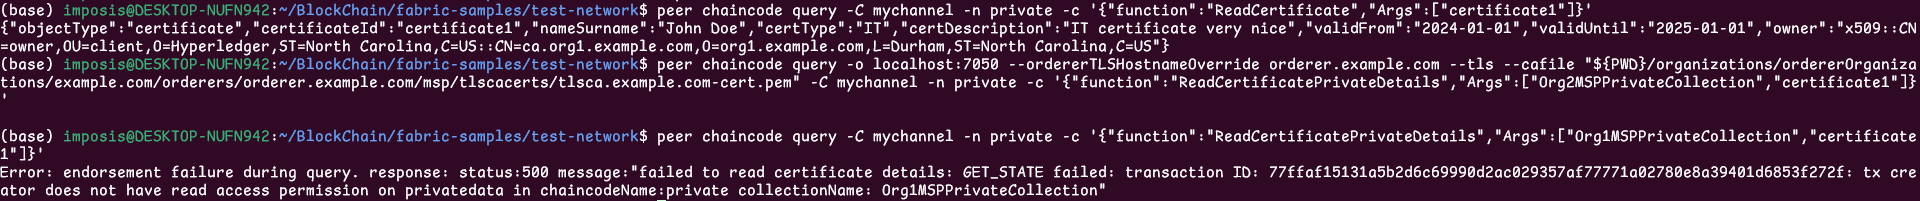
\includegraphics[width=\textwidth]{imgs/reading_certificate_org2.PNG}
    \caption{Reading certificate Org2}
    \label{fig:readingcertificate}
\end{figure}

The public data is also returned correctly.
When \texttt{ReadCertificatePrivateDetails} is called with the private collection of Org2 we can see that the response is empty as the certificate is not stored in the private collection of Org2.
When \texttt{ReadCertificatePrivateDetails} is called with the private collection of Org1 as member of Org2 we can see that an error is returned as the user is not authorized to access the private data of Org1.

\subsection{Changing certificate valid until}

\begin{lstlisting}[language=bash]
peer chaincode invoke -o localhost:7050 --ordererTLSHostnameOverride orderer.example.com --tls --cafile "${PWD}/organizations/ordererOrganizations/example.com/orderers/orderer.example.com/msp/tlscacerts/tlsca.example.com-cert.pem" -C mychannel -n private -c '{"function":"ChangeCertificateValidUntil","Args":["certificate1", "2026-01-01"]}'
peer chaincode query -C mychannel -n private -c '{"function":"ReadCertificate","Args":["certificate1"]}'
\end{lstlisting}

\begin{figure}[H]
    \centering
    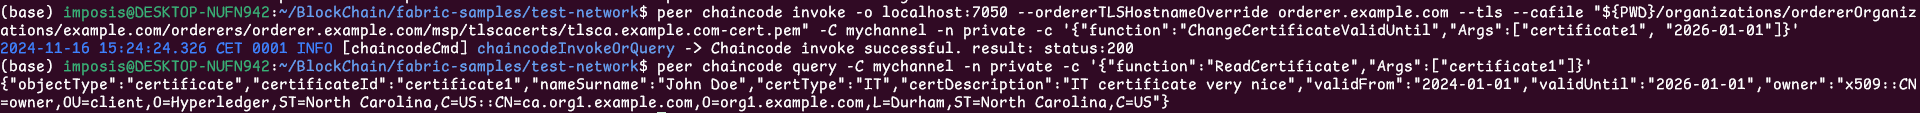
\includegraphics[width=\textwidth]{imgs/changing_validity.PNG}
    \caption{Changing valid until}
    \label{fig:changingvaliduntil}
\end{figure}

As we can see the validity of the certificate was changed.
The validUntil can be both increased or decreased.
The only condition is that the new validity must be greater than the validFrom value of the certificate.

\subsection{Certificate removal}

\begin{lstlisting}[language=bash]
peer chaincode invoke -o localhost:7050 --ordererTLSHostnameOverride orderer.example.com --tls --cafile "${PWD}/organizations/ordererOrganizations/example.com/orderers/orderer.example.com/msp/tlscacerts/tlsca.example.com-cert.pem" -C mychannel -n private -c '{"function":"RemoveCertificate","Args":["certificate1"]}' --peerAddresses localhost:7051 --tlsRootCertFiles "${PWD}/organizations/peerOrganizations/org1.example.com/peers/peer0.org1.example.com/tls/ca.crt"
\end{lstlisting}

\begin{figure}[H]
    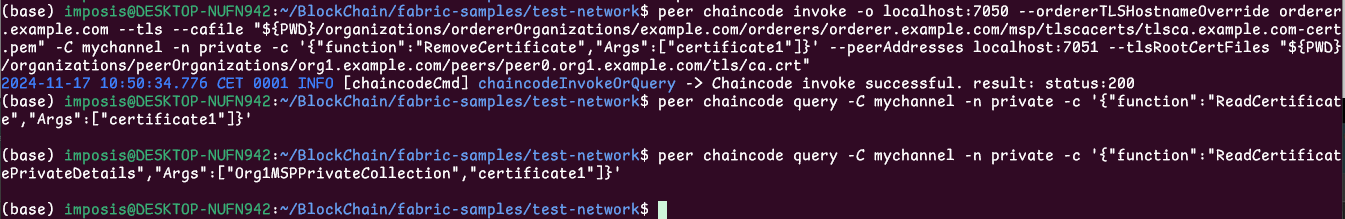
\includegraphics[width=\textwidth]{imgs/removing_certificate_and_checking_if_exists.PNG}
    \caption{Removing certificate}
    \label{fig:removingcertificate}
\end{figure}

As we can see the certificate was removed from both the public collection, which is shared between all organizations, and the private collection of the organization that issued the certificate.

\end{document}
